\documentclass[11pt]{article}
\usepackage[margin=1in]{geometry}
\usepackage{hyperref}
\usepackage{enumitem}
\usepackage{graphicx}
\usepackage{microtype}

\begin{document}
\raggedright
\raggedbottom

\title{Evidence Provenance and Unsupported-Claim Suppression in Retrieval-Augmented Generation: A Benchmark-Design Proposal}
\author{}
\date{}
\maketitle

\begin{abstract}
This brief proposes a benchmark-design study on evidence provenance and unsupported-claim suppression in retrieval-augmented generation (RAG). The research question concerns whether RAG systems can be evaluated on traceable, source-verifiable claims, and whether evidence-gated retrieval reduces the unsupported-claim rate relative to plain retrieval. The contribution is framed as a benchmark-design proposal, not a demonstrated result. No RAG-specific paper was supplied; the argument rests on an analogy from causal-reasoning benchmark criteria.
\end{abstract}

\section{Introduction}
Retrieval-augmented generation (RAG) systems are often expected to ground their outputs in retrieved evidence. However, the provenance of individual claims---whether each claim is supported by a cited span---is rarely evaluated in a systematic way. This brief motivates evidence provenance and unsupported-claim suppression as evaluation targets. It states explicitly that no RAG-specific paper was supplied for this brief, and that the argument rests on an analogy from causal-reasoning benchmark criteria. The proposed work is therefore a benchmark-design proposal, not a completed study.

\section{Related work}
The supplied evidence consists of three papers. The first is a causality-benchmark review. Its human-confirmed abstract states that many existing benchmarks for large language model causal inference and reasoning can likely be solved through retrieval of domain knowledge, which the review says questions whether those benchmarks achieve their intended purpose (claim \path{claim.review-retrieval-shortcut}; evidence \path{paper-50abf243f9f4e962403b}; confidence 0.9). The same review reports that recent benchmarks move toward a more thorough definition of causal reasoning by incorporating interventional or counterfactual reasoning, and that it derives a set of criteria a useful benchmark should satisfy; the abstract does not enumerate those criteria, so any operational checklist derived from them is an extrapolation (claim \path{claim.review-interventional-criteria}; evidence \path{paper-50abf243f9f4e962403b}; confidence 0.85). The approved Paired Intervention Provenance Suite (PIPS) frames its design rationale as an analogy from the review's interventional/counterfactual benchmark criteria to claim-level provenance; the analogy is an author-level proposal and no supplied material demonstrates that this transfer holds (claim \path{claim.pips-analogy-is-proposal}; evidence \path{paper-50abf243f9f4e962403b}; confidence 0.4).

The second paper concerns cyber threat attribution. Its human-confirmed abstract proposes a modular architecture that can combine concrete attributors via opinion pools, including a Pairing Aggregator that sequentially applies logarithmic and linear opinion pools, and reports experimental validation suggesting the modular approach does not decrease performance and can enhance precision and recall relative to monolithic alternatives (claim \path{claim.threat-attribution-modular-pools}; evidence \path{paper-bcc49f7513ed61be3a1f}; confidence 0.85). The third paper concerns distributed attribute representations. Its human-confirmed abstract proposes a third-order multiplicative model in which word context and attribute vectors interact to predict the next word, and reports experimental tasks including sentiment classification, cross-lingual document classification, and blog authorship attribution (claim \path{claim.attribute-representation-model}; evidence \path{paper-b2b2f01594862b01e12f}; confidence 0.85). These two papers are relevant to the direction only by analogy (attributor aggregation and attribute-conditioned representations); neither abstract addresses retrieval-augmented generation provenance, so their bearing on claim-to-source traceability is unverified (claim \path{claim.related-work-relevance-unverified}; evidence \path{paper-bcc49f7513ed61be3a1f}, \path{paper-b2b2f01594862b01e12f}; confidence 0.5).

\section{Method}
We propose the Paired Intervention Provenance Suite (PIPS). The paired-item schema consists of a claim, a cited span, and the surrounding evidence. Three interventions are applied: delete (remove the cited span), contradict (replace the cited span with a contradictory statement), and distractor (replace the cited span with an irrelevant but plausible span). A meaning-preserving placebo arm perturbs the prompt without altering evidence content. A scoring harness computes the pre-registered metrics. A human annotation protocol assigns `supported-by-cited-span' labels. PIPS is a design proposal; its design rationale is analogical (see claim \path{claim.pips-analogy-is-proposal}).

\section{Planned experiments}
The approved experiment plan compares evidence-gated retrieval against plain retrieval on the unsupported-claim rate. The configuration file is \path{configs/evidence_gate.yaml}. The status is planned. No run has been executed, and no unsupported-claim-rate result exists. This section is presented strictly as a plan with no results.

\section{Metrics and analysis plan}
The pre-registered metrics are: intervention-sensitivity, claim-flip, citation-redirection, placebo-adjusted sensitivity, and discriminative-gain. Directions and effect sizes for every metric are unconfirmed guesses that may not be confirmed by experiments.

\section{Limitations and open items}
\begin{itemize}[leftmargin=*,noitemsep,topsep=2pt]
\item No retrieval-augmented generation paper was supplied; the three available papers concern causal-reasoning benchmarks, cyber threat attribution, and distributed attribute representations, so no direct evidence supports RAG claim-provenance mechanisms.
\item The core analogy from interventional/counterfactual causal-reasoning criteria to claim-level provenance benchmarking is an unvalidated author proposal and may not transfer.
\item The review's derived benchmark criteria are described only at abstract level and are not enumerated in the supplied evidence, so any operational checklist is extrapolation.
\item The experiment is status planned with a human-approved plan only; no run has been executed and no unsupported-claim-rate result exists.
\item The experiment plan requires conversion to a structured Experiment Run, explicit approval, and execution under the experiment.execute capability, which is not granted in this context.
\item The evaluation dataset is described only as a `held-out evaluation set of evidence-attribution questions'; its identity, size, snapshot or version, source path, license, split policy, and access restrictions are \path{AUTHOR_INPUT_NEEDED}.
\item No code artifact, environment specification, dependency lockfile, deterministic seed, or preprocessing artifact was supplied, so reproducibility cannot be assessed or claimed.
\item Ground-truth `supported-by-cited-span' labels are expected to be contestable and annotator disagreement could dominate the intervention-sensitivity signal.
\item The intervention may perturb the prompt in ways unrelated to evidence content, risking false evidence-sensitivity; the placebo arm is intended to address this but is itself untested.
\item All supplied paper metadata is incomplete: venue, venueLevel, peerReviewed, citationCount, hasCode, doi, and metadataUpdatedAt are null, and all three records are arXiv preprints with a single source record, so peer-review status and citation impact are unverified.
\item Effect direction and size for every pre-registered metric are guesses that may not be confirmed by experiments.
\item No statistical design facts are available, including unit of analysis, number of items, repetitions or seeds, uncertainty summary, test or model, multiple-comparison handling, and exclusion or missing-data rules; these are \path{AUTHOR_INPUT_NEEDED}.
\end{itemize}

\section{Data and code availability}
No benchmark items, dataset snapshot, license, seed, environment, or code artifact was supplied. All such facts are \path{AUTHOR_INPUT_NEEDED}.

\section{Conclusion}
This brief is a proposal. No claim of effectiveness, novelty, or reproducibility can be made. The human decisions required before any such claim include: approve the experiment run and provide the structured Experiment Run; provide the dataset identity, size, snapshot or version, source path, license, split policy, and access restrictions; provide a code artifact, environment specification, dependency lockfile, deterministic seed, and preprocessing artifact; specify the statistical design (unit of analysis, number of items, repetitions or seeds, uncertainty summary, test or model, multiple-comparison handling, and exclusion or missing-data rules); resolve the annotation protocol and label contestability; validate the analogy from causal-reasoning criteria; obtain RAG-specific evidence; enumerate the review's benchmark criteria; and verify peer-review status, venue, citation counts, code availability, and DOI for the supplied papers.

\section*{Unverified Claims}
\begin{itemize}[leftmargin=*,noitemsep,topsep=2pt]
\item Unverified: that PIPS intervention-sensitivity scores discriminate evidence-grounded attribution from parametric-memory citation; no experiment has been run.
\item Unverified: that evidence-gated retrieval reduces unsupported-claim rate relative to plain retrieval; this is a planned comparison with no results.
\item Unverified: that a corpus of RAG items with verifiable claim-to-span support can be assembled at acceptable annotation cost.
\item Unverified: that claim and citation changes under evidence intervention are observable and stable enough to score.
\item Unverified: that the review's interventional/counterfactual criteria transfer from causal-reasoning benchmarks to provenance benchmarks.
\item Unverified: any claim of novelty, state-of-the-art performance, causality, or reproducibility for the proposed method.
\item Unverified: that the cyber threat attribution modular opinion-pool architecture or the distributed attribute representation model provides direct support for RAG provenance; their use here is analogical only.
\item Unverified: peer-review status, venue, citation counts, code availability, and DOI for any supplied paper, all of which are null in the supplied metadata.
\end{itemize}

\appendix
\section*{Illustrative Figures}
The figures in this appendix illustrate the tooling that produced this brief, not the research subject. They are not results.

\begin{figure}[htbp]
\centering
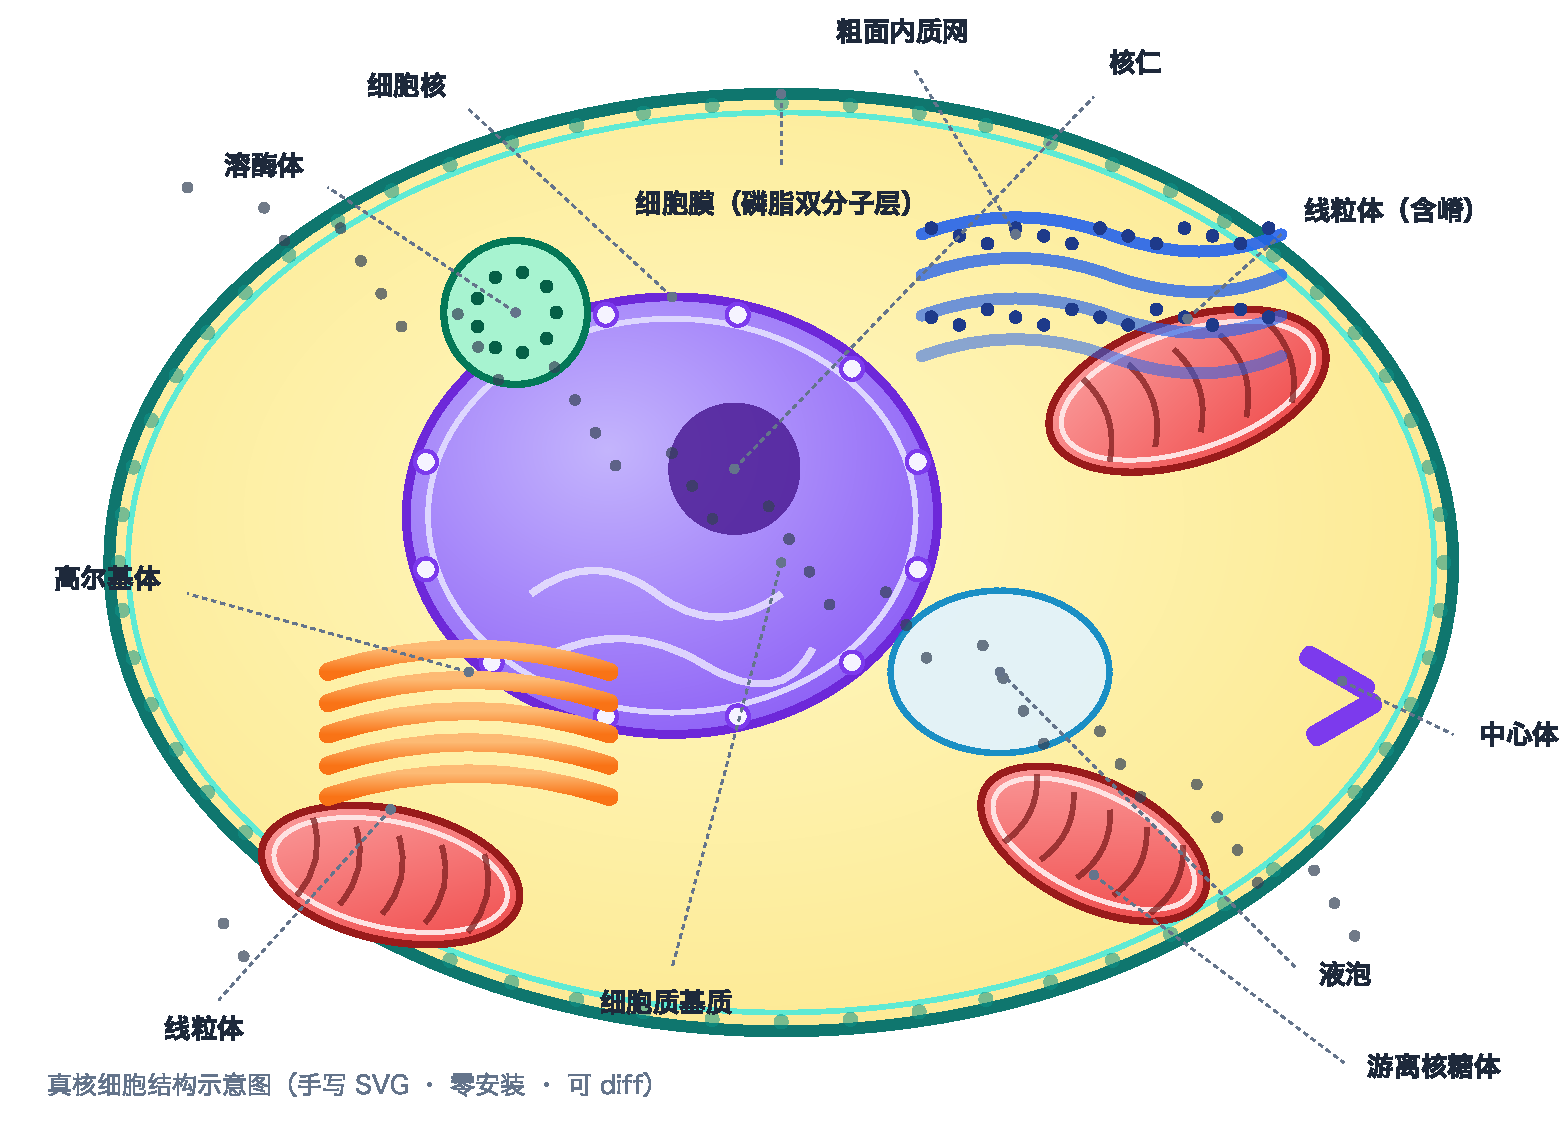
\includegraphics[width=0.98\linewidth]{figures/cell-structure.pdf}
\caption{The cell-structure diagram generated by the tooling that produced this brief.}
\end{figure}

\begin{figure}[htbp]
\centering
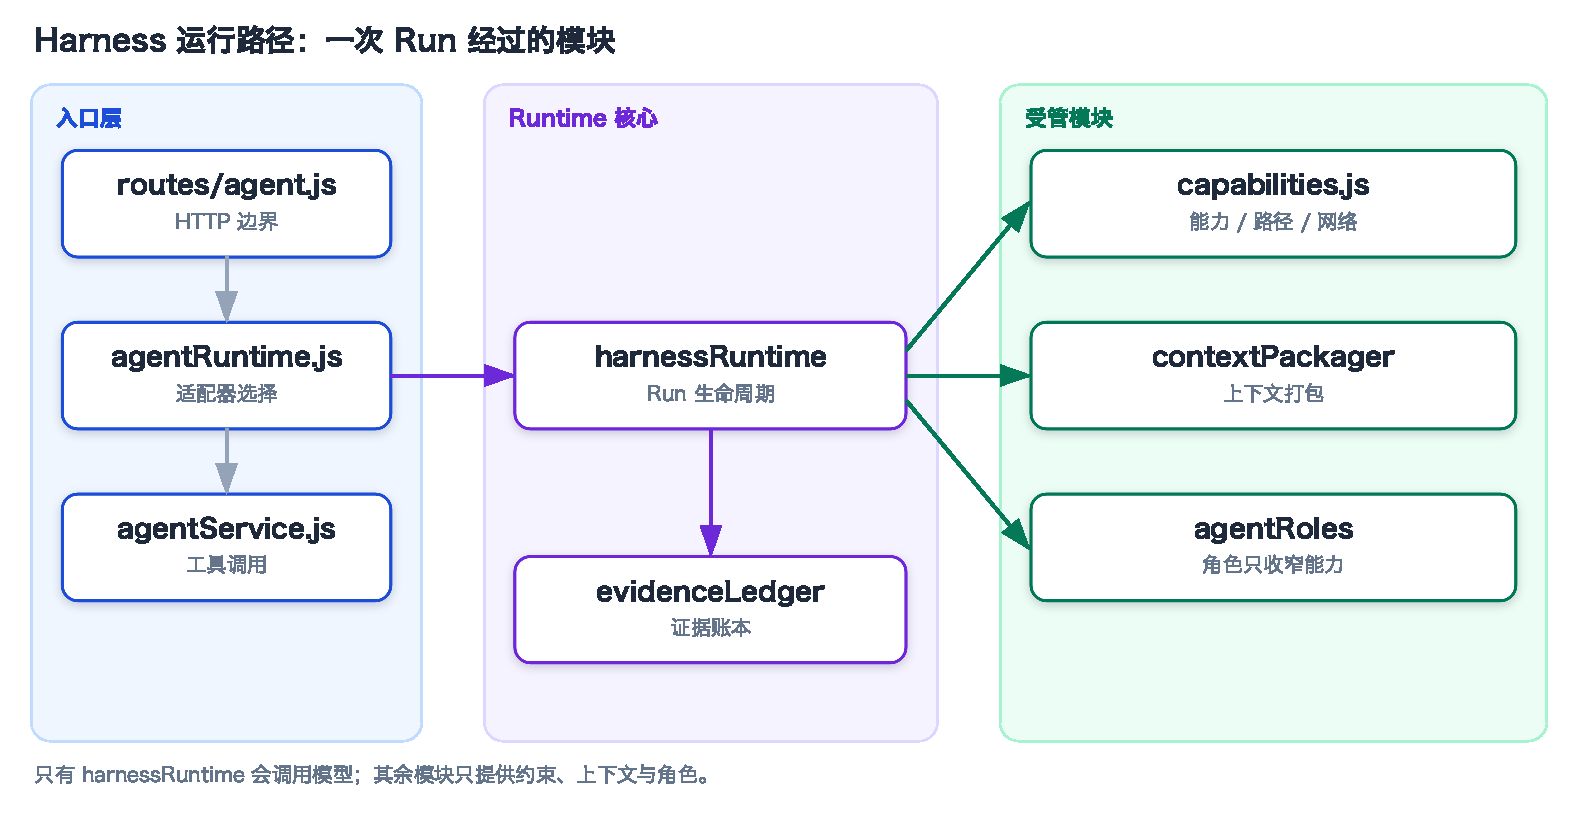
\includegraphics[width=0.80\linewidth]{figures/module-graph.pdf}
\caption{The module-graph diagram generated by the tooling that produced this brief.}
\end{figure}

\begin{figure}[htbp]
\centering
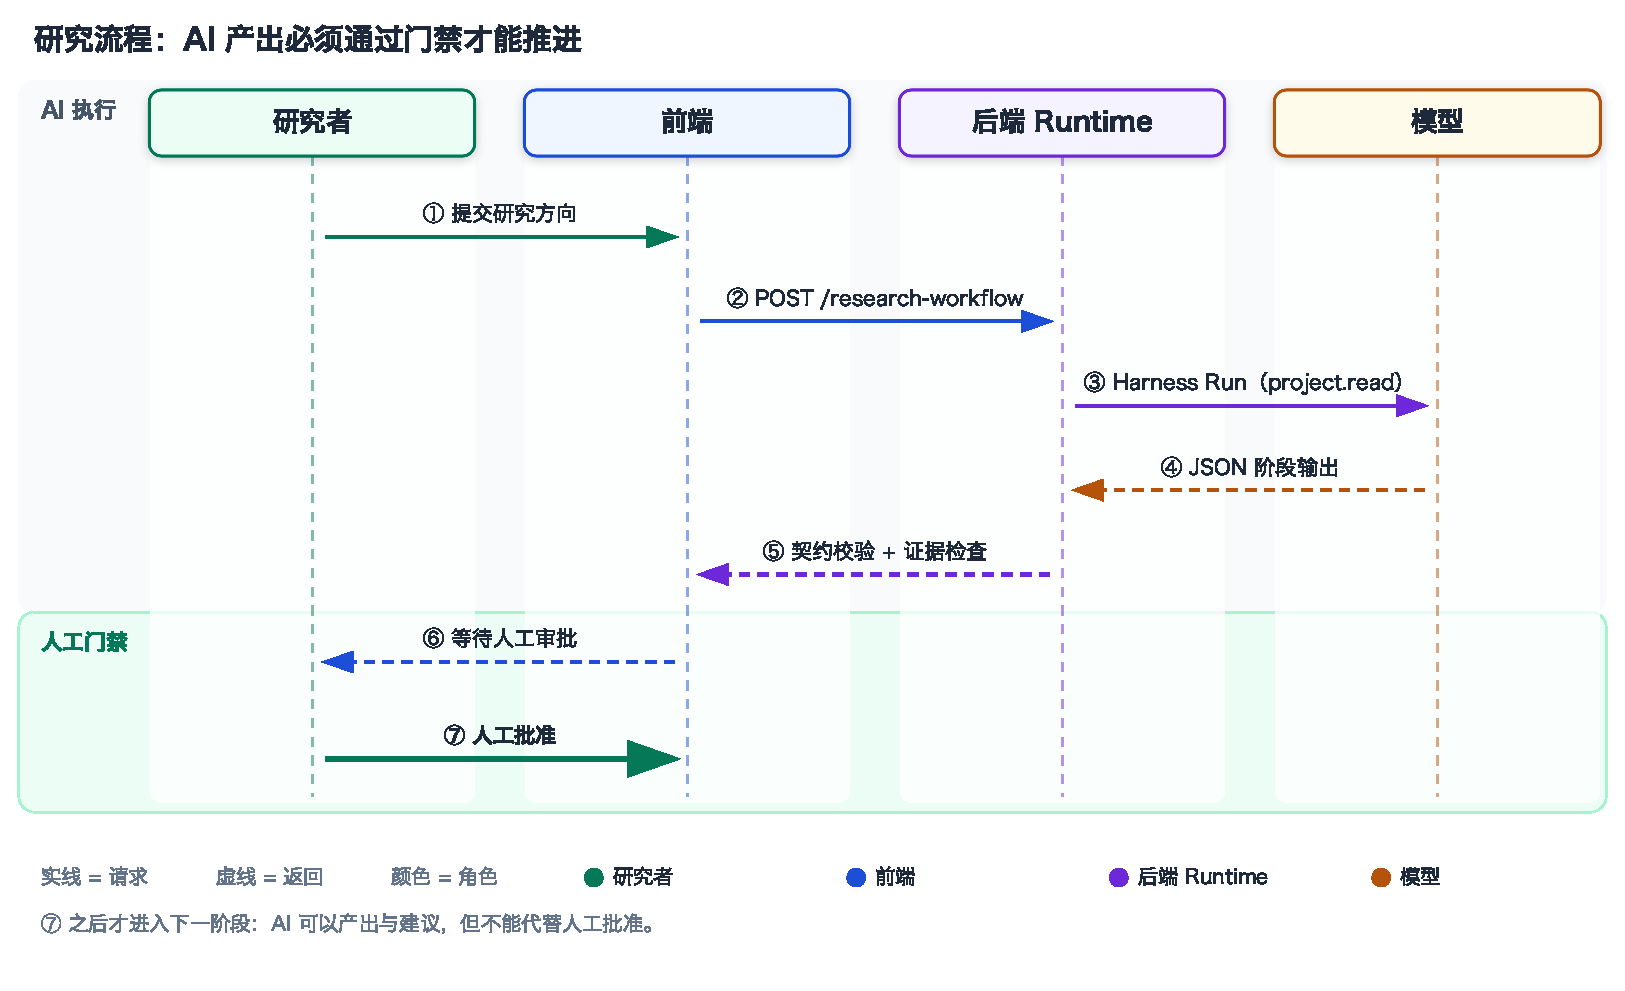
\includegraphics[width=0.86\linewidth]{figures/sequence-flow.pdf}
\caption{The sequence-flow diagram generated by the tooling that produced this brief.}
\end{figure}

\begin{figure}[htbp]
\centering
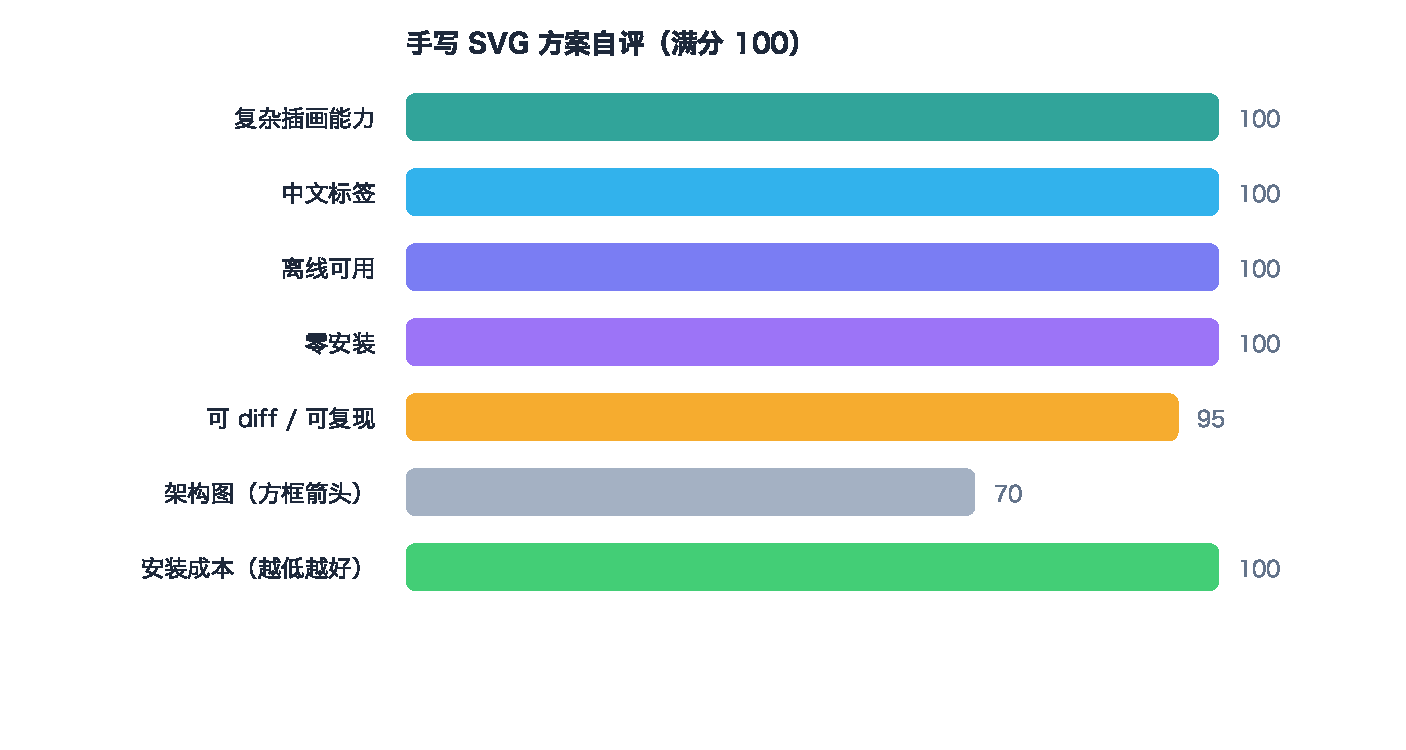
\includegraphics[width=0.72\linewidth]{figures/comparison-chart.pdf}
\caption{The comparison-chart diagram generated by the tooling that produced this brief.}
\end{figure}

\end{document}
